\documentclass[11pt,a4paper]{report}
\usepackage[utf8]{inputenc}
\usepackage{amsmath}
\usepackage[pdftex]{graphicx}
% declare the path(s) where your graphic files are
\graphicspath{{./png}}
\usepackage{subfigure}
%\usepackage{tabularx}
%\usepackage{adjustbox}
%\usepackage[colorinlistoftodos]{todonotes}
%\usepackage{csquotes}
%\usepackage{comment}
%\usepackage{imakeidx}
%tabela
%\usepackage{multirow}
%\usepackage{xcolor}
\usepackage[margin=3cm]{geometry}
\usepackage{hyperref} %to show links
\usepackage[toc,acronym,nopostdot,nonumberlist]{glossaries}
\usepackage{titling}
%\usepackage{tikzpagenodes}
\usepackage[ddmmyyyy]{datetime}
\usepackage{setspace}
%\usepackage{indentfirst}

%para definir a localização das tabelas e imagens em modo strict
%\usepackage{placeins}

\usepackage{biblatex}
\addbibresource{ref.bib}
\makeglossaries

%colocar aqui variáveis que serão utilizadas no texto:
\newcommand\kbps{\text{\textit{k}bit/s}}
\doublespacing

\begin{document}

\begin{titlepage}
\centering
\vspace{8cm}
\huge Lab Report for Peak Detector \\
\vspace{2cm}
%\large a project authored by\\
\large a lab assignment report authored by\\
\Large Bowen Zhang, Weifeng Du, \par Zixuan Luan, Yanyan Ge\\
\vspace{4cm}
\large supervised by\\
\large Dr. Shuangyi Yan,\par Dr. Scott Tancock,\par Dr. Tony Horseman\\
\vspace{2cm}
\newdateformat{daymonthyear}{\THEDAY\ \monthname[\THEMONTH], \THEYEAR}
\daymonthyear\today \\
%December, 2019
%\large v2.3
\end{titlepage}

%%%%% colocar aqui acrónimos
\newacronym{ersc}{ERSC}{Engenharia de Redes e Sistemas de Computadores}
\newacronym{wn}{WN}{Wireless Network}
%\textbf{Keywords:} word1. word2. word3. word4.
%insert index
\tableofcontents
\glsaddall
%\printglossary[type=\acronymtype]
%\printglossary[type=main,title={Glossary},toctitle={Glossary}]
%%%%%%%%%%%%%%%%%%%%%%%%%%%%%%%%%%%%%%%%%%%%%%%%%%%%%  

\chapter{Group Composition and Task Division}
\label{chap:Group Composition and Task Division}

In this chapter, we describe the group composition and task division
among group members as well as the statement of each team member on their contribution to the project.

\section{Group Composition} 
\label{sec:Group Composition}
We are group 2 and our group members including Bowen Zhang, Weifeng Du, Zixuan Luan and Yanyan Ge. Bowen Zhang and Weifeng Du are in lab group A, while Zixuan Luan and Yanyan Ge are belong to lab group B.

We shall deal with the signed peak detector because our group number is even. We divided the whole group into two teams for two separate parts of the project. Team A including Bowen Zhang and Weifeng Du works on the design and implement of Command Processor. Team B including Zixuan Luan and Yanyan Ge works on the design and implement of Data Processor.

\section{Task Division}
\label{sec:Task Division}


Task division for Team A:




Task division for Team B:

~\\Work together part:

Design the ASM chart before programming on Vivado. 
After finishing the separate parts, do the Stand-alone simulation for the Data Processor and debug.


~\\Zixuan Luan: 

Design the ANNN: Detect the request comes from Command Processor and fetch required number of data from Data Generator by reading ctrlIn and writing ctrlOut base on the two phase signaling protocol. 

~\\Yanyan Ge:

Desing the L and P part: Design the algorithm based on the observation on the simulation of the given synthesised version of signed Data Processor. Tackle the condition of comparing signed values and assign them to the the dataResults in proper sequence.


\chapter{Project Plan}
\label{Project Plan}

In this charper, we describe the overall project plan for Team 1 and Team 2 separately, including a diagrammatic
work plan, Gantt chart, including the timelines, milestones as well as team or group meeting.

\section{Plan for Team A}
\label{sec:Plan for Team A}

We started the project from 17th February 2020 and end the project on 17th April 2020. 

On the first week (16th week), we took an overview on the given materials on the assignment, project function and the use of Vivado. Then we had a meeting on task division next Monday and came up with a roughly task division plan, then for the next few days of the 17th week, our team analysed the project and roughly worked out the ASM chart.

From 29th Feb. to 9th Mar, Zixuan Luan started to work on the communication between Data Generator and Data Processor as well as the ANNN part. From 3rd to 12th, Yanyan Ge started to work on designing the part of P and L. On 10th, our team had a meeting on reporting the ANNN task. From 11st to 18th, Zixuan started to optimize and debug the communication part. From 13rd to 21st, Yanyan Ge started to merge the ANNN part by Zixuan and the P and L part she designed before. From 22nd to 31st, the whole team worked together to do the final stand-alone simulation for the Data Processor, debugging and optimizing the whole work. 

From 1st April to 4th April, the whole group worked on the final integration between the Data processor and Command Processor. And on 5th April, we had a meeting on report writing. Finally, we started to work on writing report till 17th April.

Figure (\ref{Team A plan}) describes the team plan in Gantt chart and the red lines in the chart show the milestones.

\begin{figure}[!ht]
    \begin{centering}
        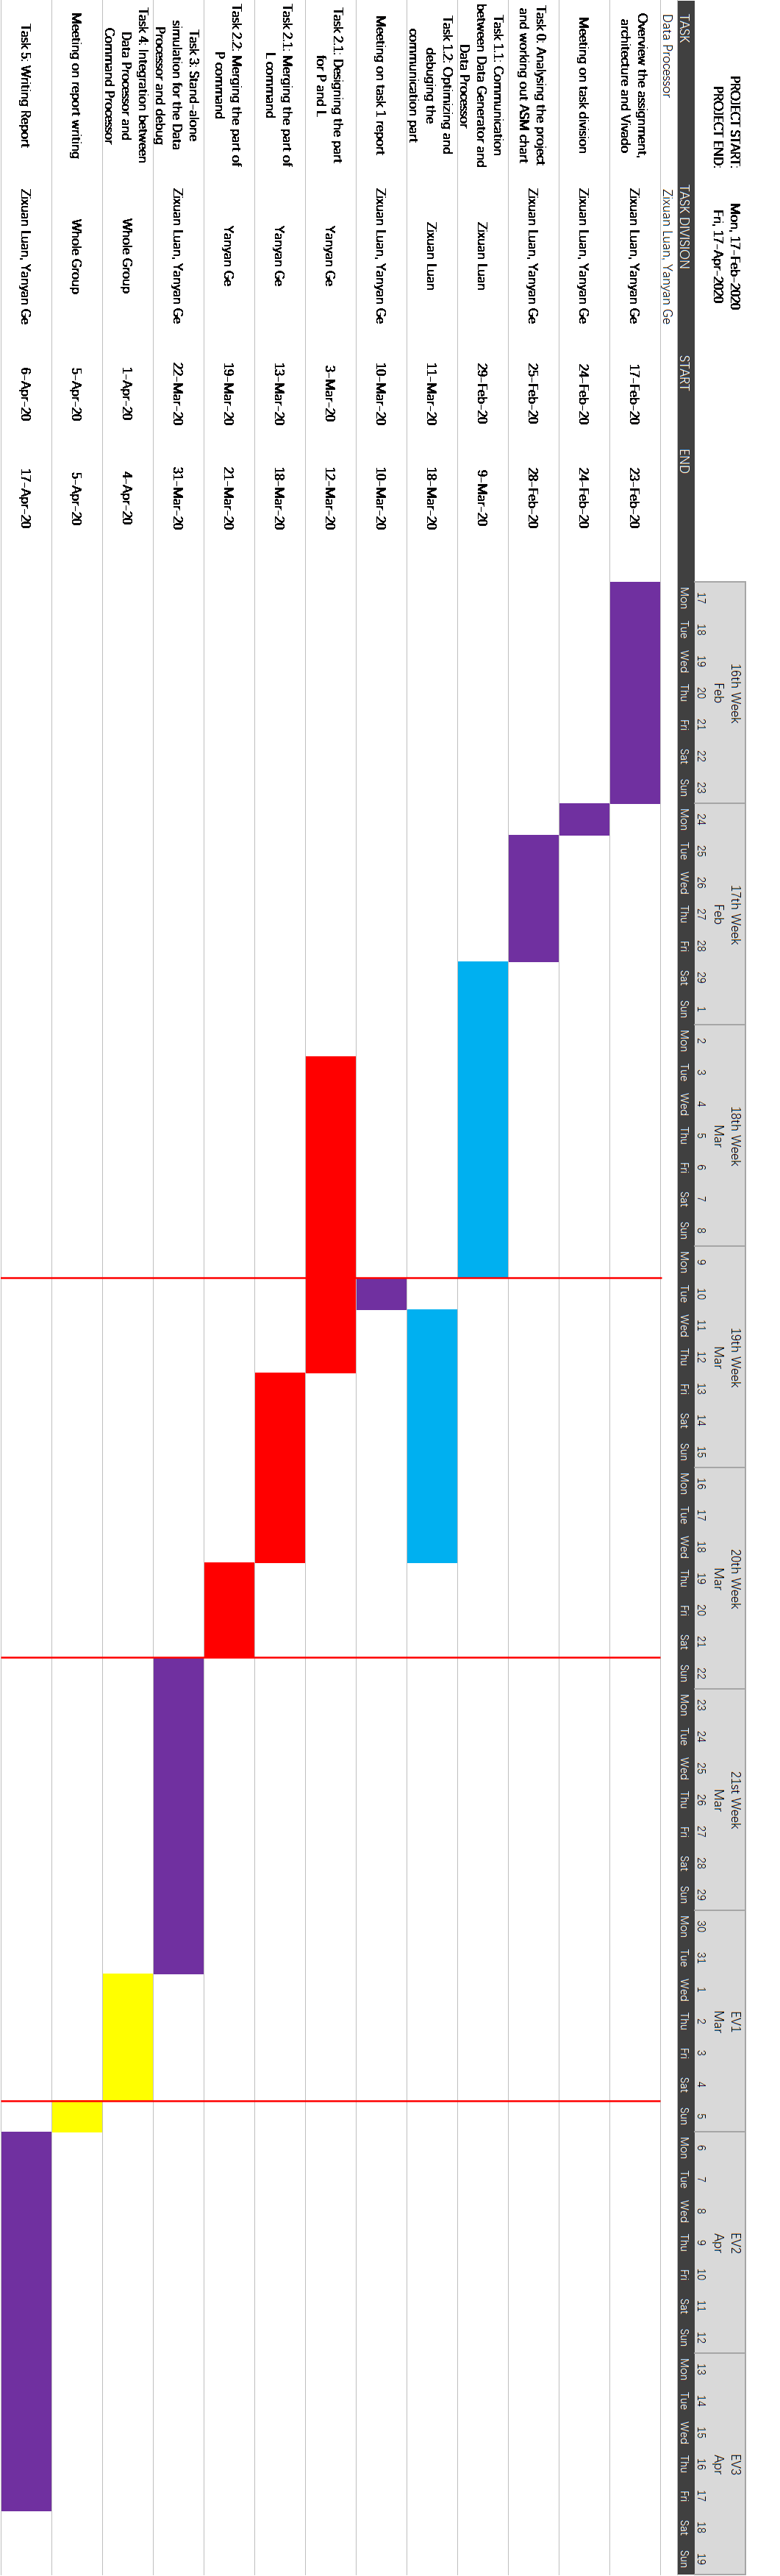
\includegraphics[scale=0.31]{TeamA_plan.png}
        \par\end{centering}   
    \caption{The whole project plan for Team A.\label{Team A plan}}
\end{figure}   

\section{Plan for Team B}
\label{sec:Plan for Team B}





%%%%%%%%%%%%%%%%%%%%%%%%%%%%%%%%%%%%%%%%%%%%%%%%%%%%%  
\chapter{Data Processing Module by Team A}
\label{cap:Data Processing Module by Team A}

We designed and implemented the Data Processor in two parts. The first part is ANNN part which needs us to read the number comes from Command Processor and return the required number of words. The second part is PL and L part which requires us to return the largest signed data as well as the six data next to it and return the index of the largest number to the Command Processor. 

\section{Part1: ANNN}
\label{sec:Part1: ANNN}

As for the first part, what we need to do first is to set up the communication between Data Generator 
and Data Processor using the two phase protocol. To realize the communication, we first determine “start = 1”
 and “curState = star\_{data}\_{gen}” to make sure the Data Processor fetches new data after the former data has been
  read and transmitted by Command Processor then we change the ctrlout signal and put the data returned from Data 
  Generator on byte. From the simulation results, we can find that it takes only one clock cycle for Data Generator
   to return a new data while it takes more time for the Command Processor to finish the serial transmit. 

We also set a counter to count the number of words that has been transmitted. We take the NNN of ANNN command as 
the final number and count up when the ctrlout signal changes and reset the counter as soon as the counter reach 
the final number. To achieve this function, we use a state machine with 4 states. INIT is used as an idle state, 
means nothing will happen until a start signal is detected. The second state is start\_data\_gen, which is used to 
communicate and count and the next one is complete\_data\_gen, which writes the data fetched from Data Generator 
on byte. The last state is complete\_all\_data\_gen, which is used to reset the counter and return “seqDone = 1” to
 Command Processor after the NNN words has been successfully fetched and transmitted.

The Block logic graph and the ASM chart of the above ANNN part is Figure ({\ref{TeamA ANNN}}) 

\begin{figure}[htbp]
    \centering
    \subfigure[The block logic graph]{
    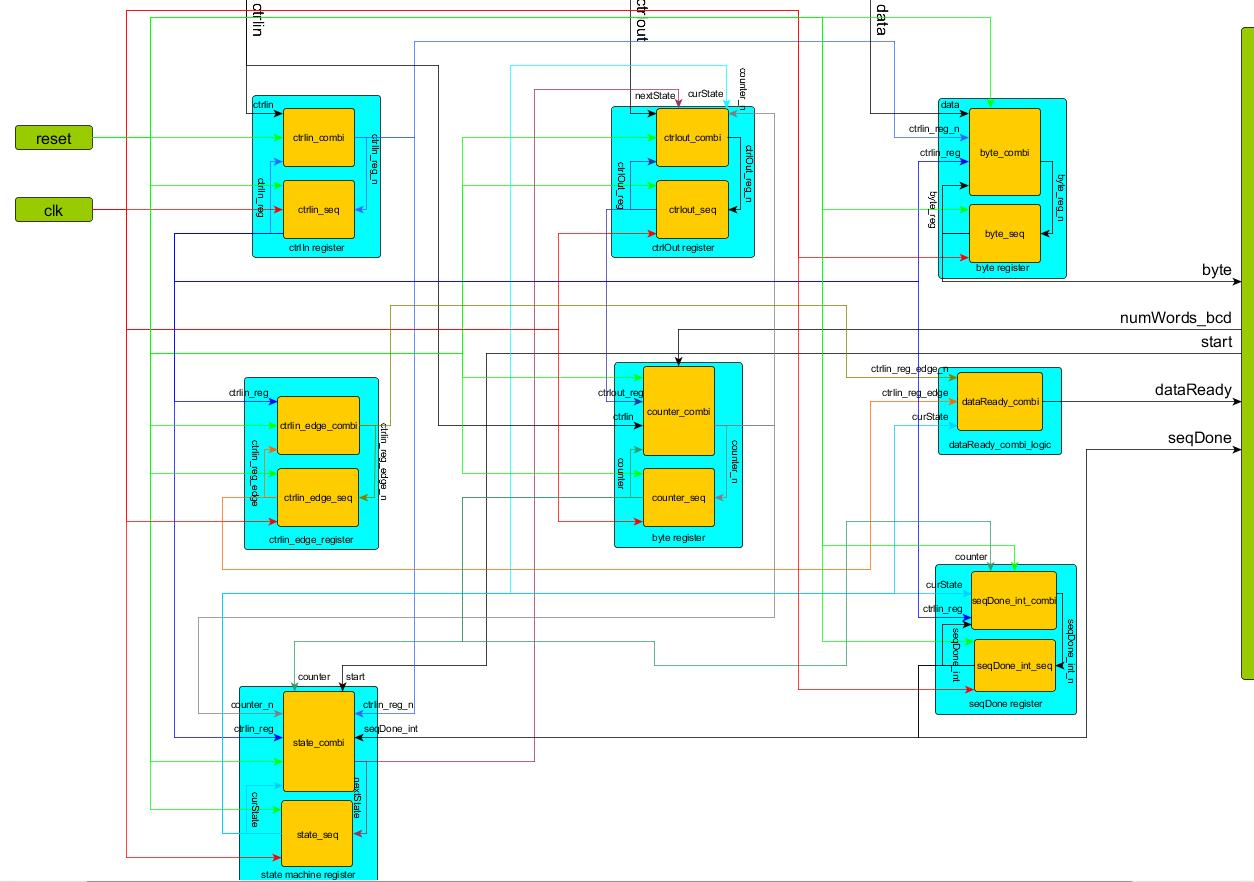
\includegraphics[width=6.7cm]{TeamA_block_ANNN.jpg}
    }
    \quad
    \subfigure[The ASM chart]{
    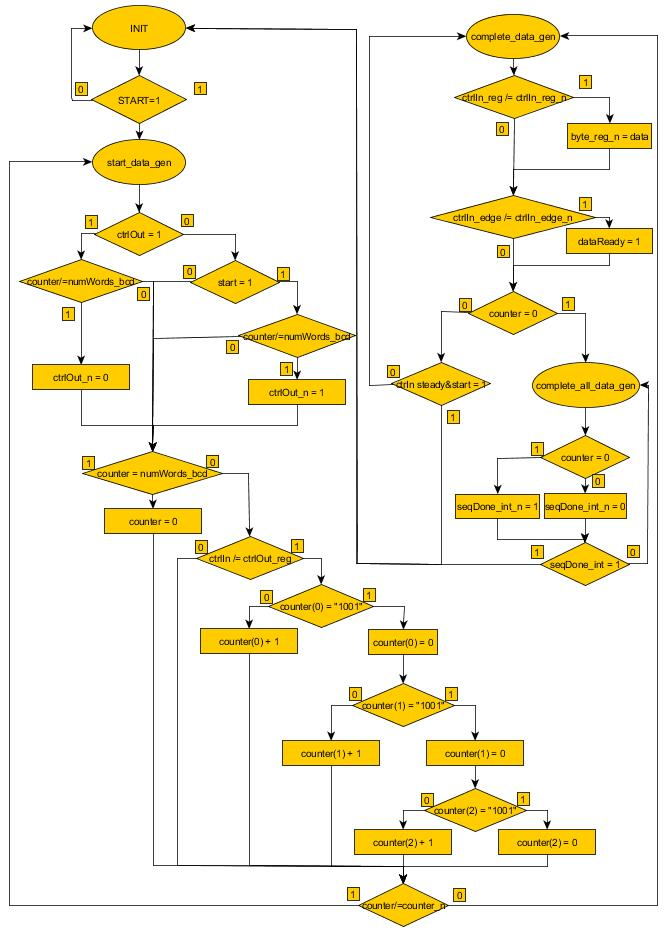
\includegraphics[width=6.7cm]{TeamA_stateANNN.jpg}
    }
    \caption{The block graph and ASM chart of ANNN part\label{TeamA ANNN}}
\end{figure}


\section{Part2: P and L}
\label{sec:P and L}

The second part is to determine the largest value and return the three numbers on both sides of it which is totally
 7 bytes of data. What we do is to set a three bytes register (datahalfside register) to record the three data 
 fetched before the current value, as soon as we determine the largest value we will substitute current middle 
 data of dataResults array with the max data and the three bytes before which with the three bytes in datahalfside 
 register and renew the last three bytes with three new bytes after the max data. And as for the maxIndex, we will
  assign it with the value of counter as soon as we find the max data.

To realize this function, we use 6 states including INIT, start\_l. L\_1 ,L\_2, L\_3, L\_4. Start\_l is a state we jump
 to when we meet the max data and we do the substitution process. L\_1 to L\_3 is the state we use to fill the first, 
 second and third bytes after the max data and L\_4 is used to keep the dataResults don’t change and record the 
 datahalfsides until the max data appears.

The Block logic graph and the ASM chart of the above P and L part is Figure (\ref{TeamA P and L})
because the structure of state L1, L2, L3 are same, we only show the ASM chart of L1

\begin{figure}[!ht]
    \centering
    \subfigure[The block logic graph]{
    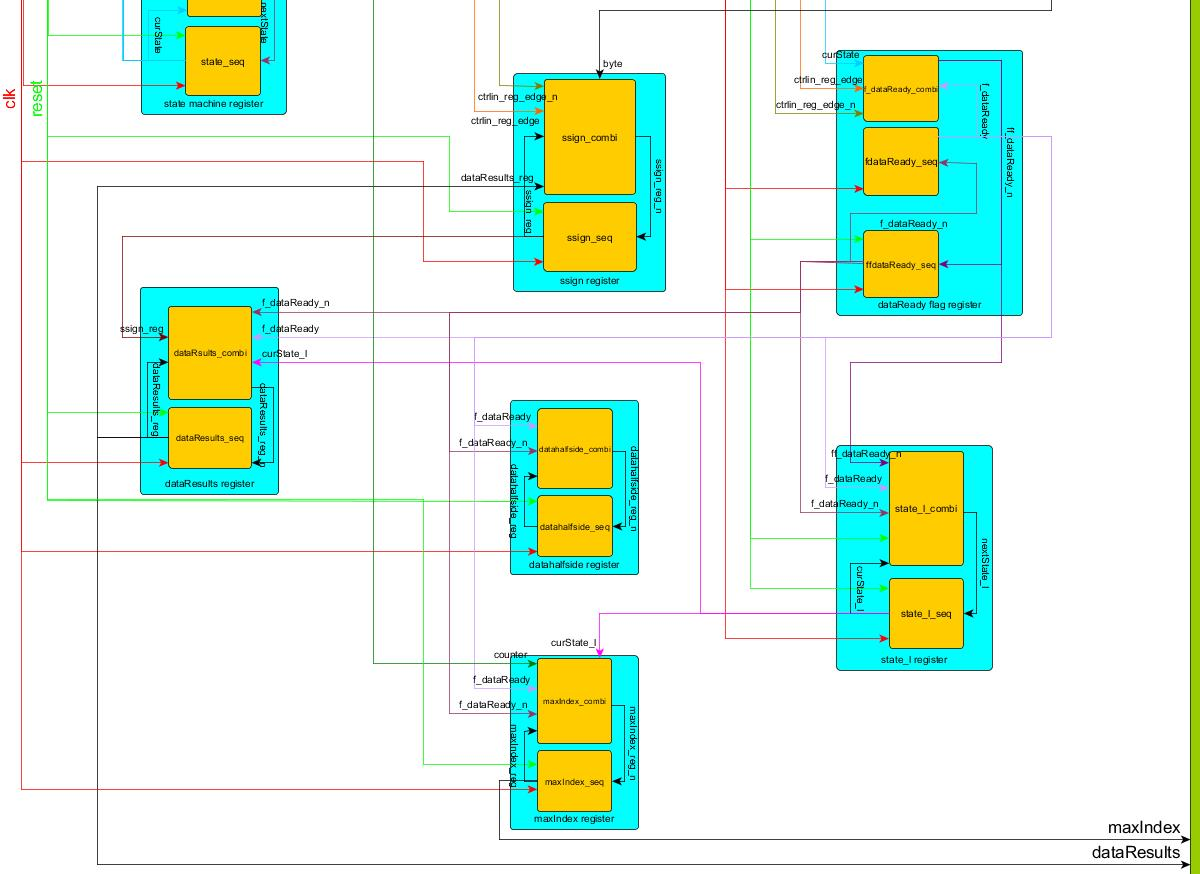
\includegraphics[width=6.7cm]{TeamA_block_PL.jpg}
    }
    \quad
    \subfigure[The ASM chart (statel)]{
    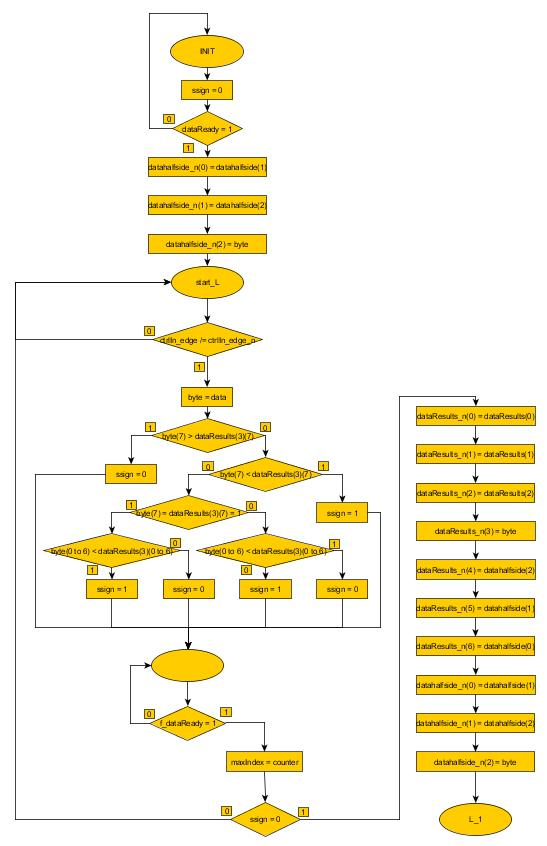
\includegraphics[width=6.7cm]{TeamA_startL.jpg}
    }
    \quad
    \subfigure[The ASM chart (L1)]{
    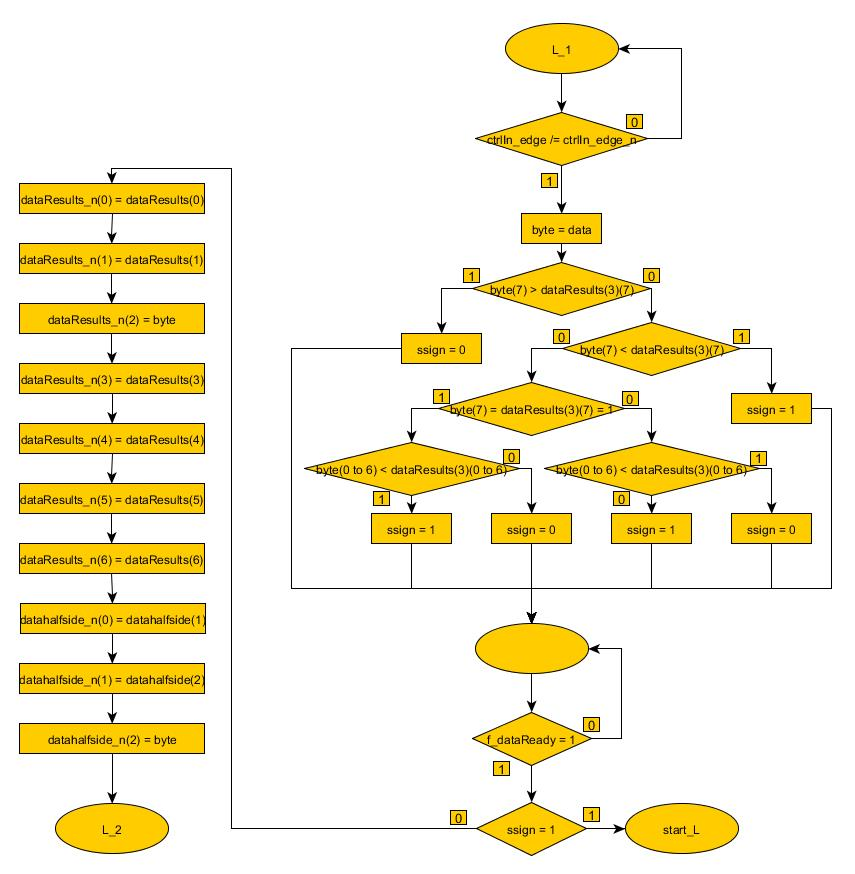
\includegraphics[width=6.7cm]{TeamA_L1.jpg}
    }
    \quad
    \subfigure[The ASM chart (L4)]{
    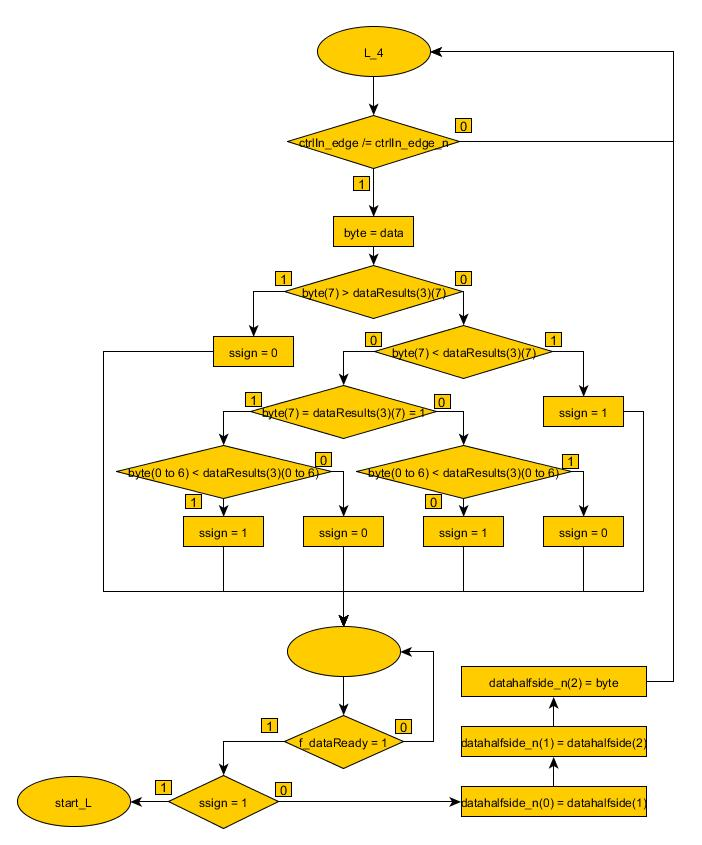
\includegraphics[width=6.7cm]{TeamA_L4.jpg}
    }
    \caption{The block graph and ASM chart of P and L part\label{TeamA P and L}}
\end{figure}

\chapter{Command Processing Module by Team B}
\label{cap:Command Processing Module by Team B}


\chapter{Simulation Results}
\label{cap:Simulation results}

\section{Simulation Results of Team A}
\label{sec:Simulation Results of Team A}

From the Figure (\ref{TeamA ANNN all})), we can find that the numWords comes from Command Processor is 12 and the Data
 Processor successfully output 12 bytes of data onto the byte signal.

\begin{figure}[!ht]
    \begin{centering}
        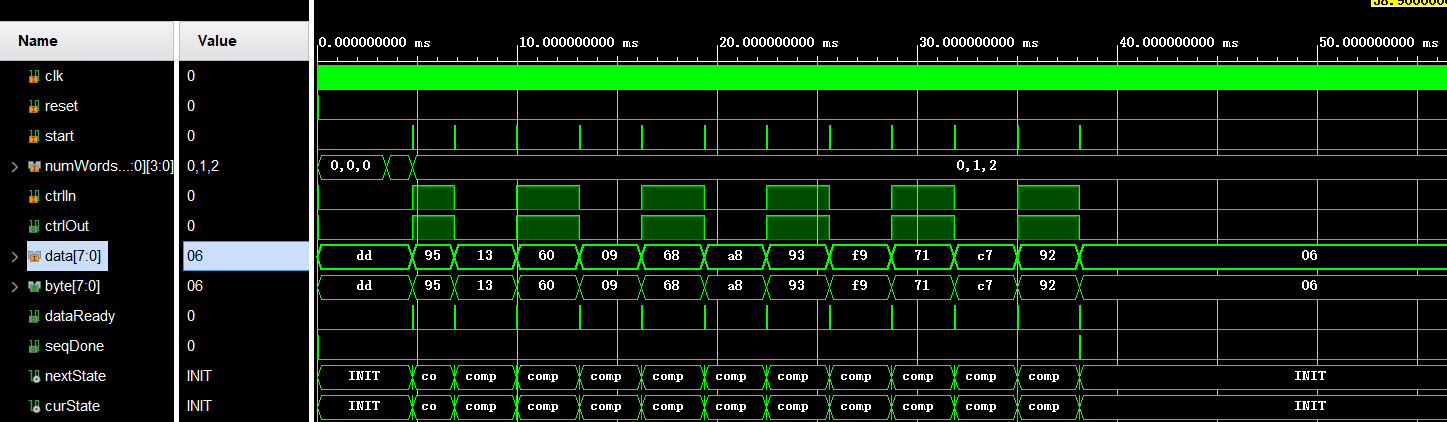
\includegraphics[scale=0.5]{TeamA ANNN all.png}
        \par\end{centering}   
    \caption{The simulation result of ANNN.\label{TeamA ANNN all}}
\end{figure}   

From the Figure (\ref{TeamA PL all}), we can find that when a new data comes Data Processor will compare it with current max 
data and decide whether change the dataResults or not. Because we are group 2, among the first series of data,
 “71” is the largest one and the dataResults is ”06, 92, c7, 71, f9, a8” which is correct. What’s more, whenever
  a larger data is detected, the maxIndex will change to the index of the new data.

\begin{figure}[!ht]
    \begin{centering}
        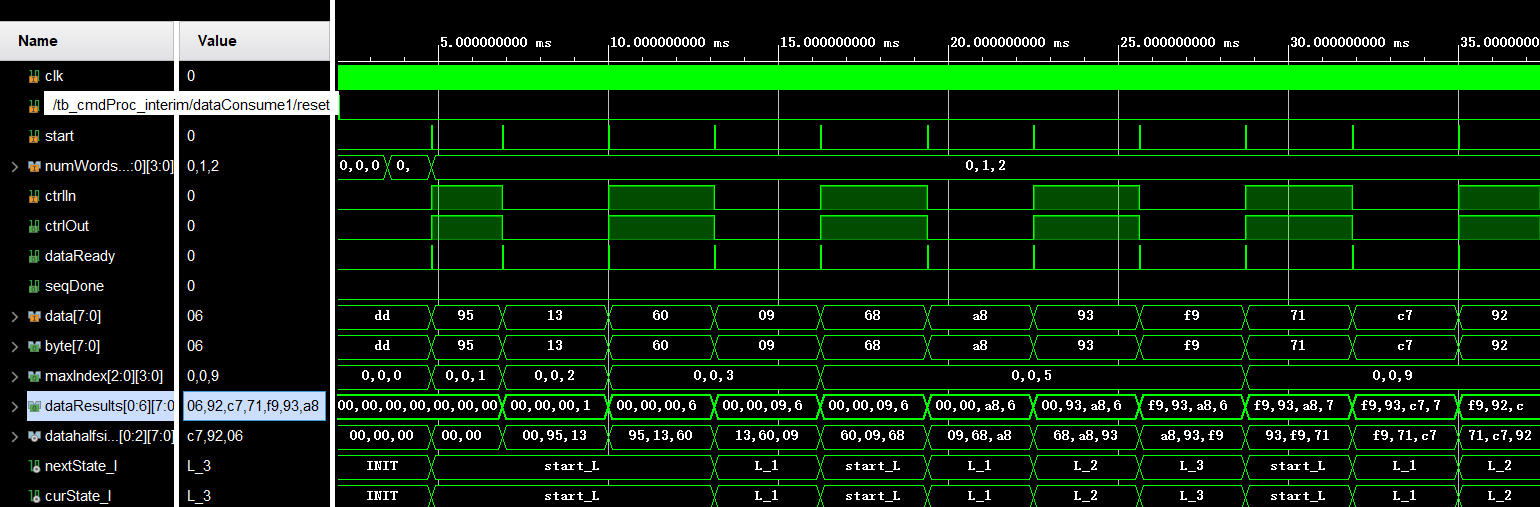
\includegraphics[scale=0.5]{TeamA PL all.png}
        \par\end{centering}   
    \caption{The simulation result of ANNN.\label{TeamA PL all}}
\end{figure}   



\section{Simulation Results of Team B}
\label{sec:Simulation Results of Team B}


\addcontentsline{toc}{chapter}{References} 
\printbibliography[title={References}]

\end{document}